\documentclass{beamer}

\usepackage[utf8]{inputenc} % Required for inputting international characters
\usepackage[T1]{fontenc}
\usepackage[french]{babel}
\usepackage{graphicx}
\usepackage{xcolor}
\usepackage{mathtools}
\usepackage{bm}
%\usepackage{enumitem}

\usepackage[autostyle=true,french=guillemets]{csquotes}

\usetheme[progressbar=frametitle,numbering=fraction,block=fill,subsectionpage=progressbar]{metropolis}
\definecolor{lightgray}{rgb}{0.95, 0.95, 0.95}
\usecolortheme{seahorse}
\setbeamercolor{alerted text}{fg=red}
% --------------------------
\title{Stochastic optimization for large scale optimal transport}
\author{Hugo Cisneros}
% \institute{
%     Mines ParisTech \\[10pt]
%     \includegraphics[height=30pt]{figures/mines-logo}
%     \hfill
%     \includegraphics[height=20pt]{figures/sorbonne-logo}
%     \hfill
%     \includegraphics[height=25pt]{figures/inria-logo}
% }
\date{January 7th, 2019}


\newcommand*\tick{\item[\includegraphics[height=10pt]{figures/tick.png}]}

% --------------------------

\begin{document}
\maketitle

\begin{frame}{Presentation of OT}
    \vfill
    Kantorovitch Formulation of regularized OT: {\scriptsize\begin{align*}\tag{$\mathcal{P}_\varepsilon$}
    \label{eq:primal}
    W_\varepsilon(\mu, \nu) &= \min_{\pi\in \Pi(\mu, \nu)} \int_{\mathcal{X}, \mathcal{Y}} c(x, y)\text{d} \pi(x, y) + \varepsilon\text{KL}(\pi|| \mu \otimes \nu) \\
    \tag{$\mathcal{D_\varepsilon}$}
    & = \max_{(u, v)\in \mathcal{C}(\mathcal{X})\times\mathcal{C}(\mathcal{Y})} \int_\mathcal{X} u(x)\text{d}\mu(x) + \int_\mathcal{Y}v(y)\text{d}\nu(y) - \iota_{U_c}^\varepsilon(u, v)\\
    \tag{$\mathcal{S_\varepsilon}$}
   & = \max_{v\in\mathcal{C}(\mathcal{Y})} H_\varepsilon(v)\triangleq \int_\mathcal{X} v^{c,\varepsilon}(x)\text{d}\mu(x) + \int_\mathcal{Y}v(y)\text{d}\nu(y) - \varepsilon
    \end{align*}}

    Sinkhorn updates: $u^{\ell+1} = \frac{\mu}{Kv^\ell} ; v^{\ell+1} = \frac{\nu}{K^Tv^{\ell+1}}$ $\rightarrow$ $O(n^2)$

    No general solver in the semi-discrete case. 

    \begin{center}
        \textbf{What about large scale ?}
    \end{center}
\end{frame}

\begin{frame}{Stochastic optimization}
    \begin{minipage}{.46\linewidth}
        \textbf{Discrete OT:}
    \end{minipage}
    \hfill
    \hfill
    \begin{minipage}{.46\linewidth}
        \textbf{Semi-discrete OT:} 
    \end{minipage}   


    \begin{minipage}{.46\linewidth}
        \begin{align*}
            W_\varepsilon(\mu, \nu) =\max_{\bm{v}\in \mathbb{R}^{J}}\sum_{i=1}^I \overline{h}_\varepsilon(x_i, \bm{v})\bm{\mu}_i
        \end{align*}

        Gradient aggregation algorithms (SAG and SAGA)

        {\footnotesize\begin{align*}
            v_{k+1} & = v_k + \texttt{step}* \left( \nabla f_i - \right.\\
            & \left. \nabla f_{[i]} + \frac{1}{I}\sum_i \nabla f_{[i]}\right)
        \end{align*}}
    \end{minipage}
    \hfill
    \vline
    \hfill
    \begin{minipage}{.46\linewidth}
        \begin{align*}
            W_\varepsilon(\mu, \nu) = \max_{v}\  \mathbb{E}_{X}[h_\varepsilon(X, v)]
        \end{align*}
        Stochastic gradient ascent

        {\footnotesize\begin{align*}
            v_{k+1} & = v_k + \frac{\texttt{step}}{\sqrt{k}}* \nabla f_i 
        \end{align*}}
    \end{minipage}
\end{frame}

\begin{frame}{Theoretical analysis}
    \textbf{Convergence rates}
    \begin{description}
        \item[Stochastic gradient] $O(1/\sqrt{k})$ for non strongly convex, $O(1/k)$ for strongly convex
        \item[SAG and SAGA] $O(1/k)$ for non strongly convex, linear for strongly convex (at the expense of storing gradients)
    \end{description}
\end{frame}

\begin{frame}{Numerical findings - Discrete OT}
    \begin{minipage}{.4\linewidth}
        \textbf{Synthetic data}
        \begin{figure}
            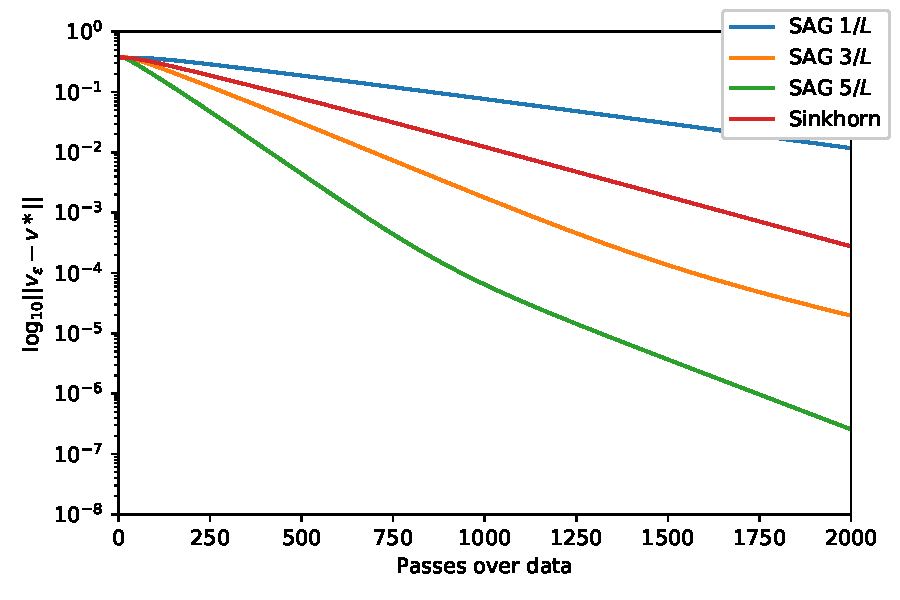
\includegraphics[width=\linewidth]{figures/lr_bench_sag.pdf}
        \end{figure}
        \begin{figure}
            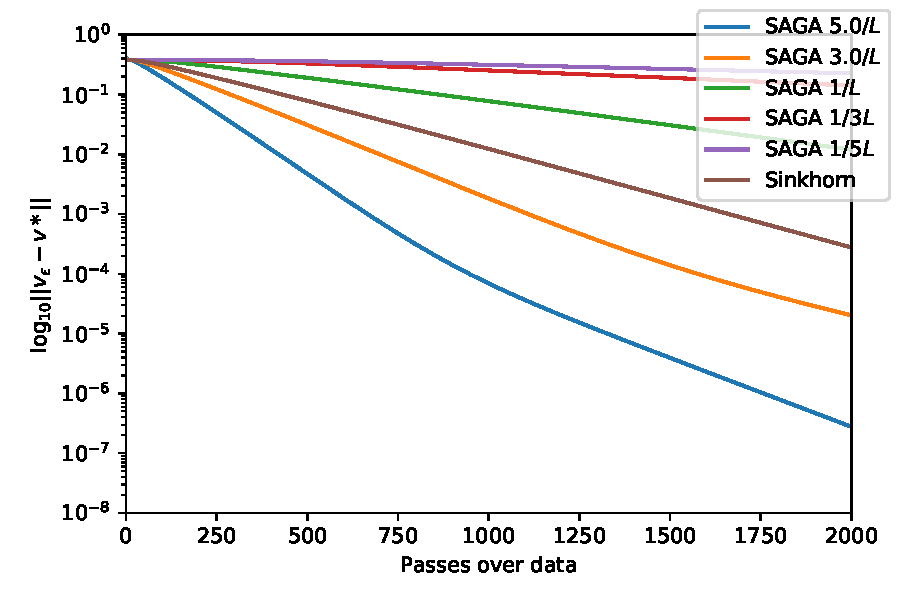
\includegraphics[width=\linewidth]{figures/lr_bench_saga.pdf}
        \end{figure}
    \end{minipage}
    \hfill
    \vline
    \hfill
    \begin{minipage}{.4\linewidth}
        \textbf{Image retrieval task}
        \begin{figure}
            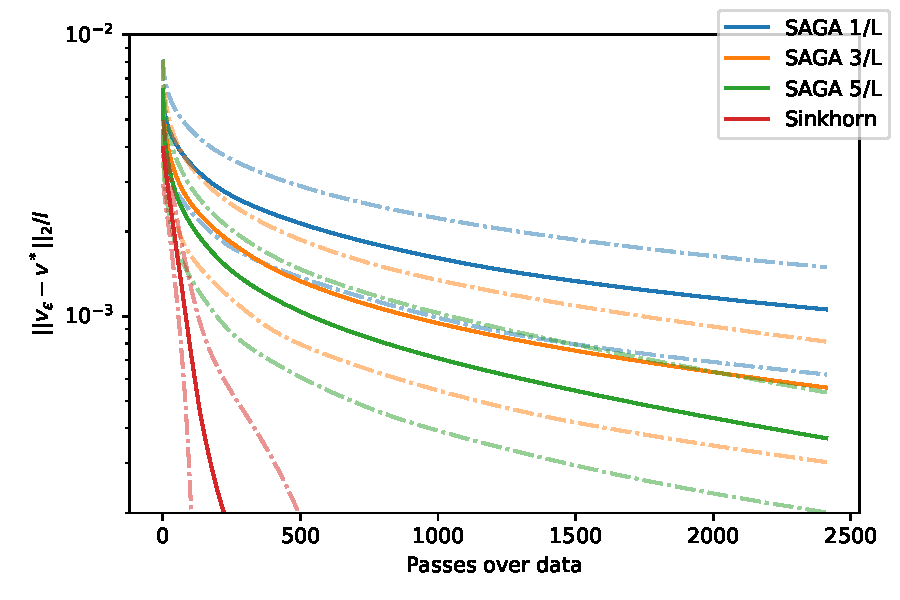
\includegraphics[width=\linewidth]{figures/sag_image_retreival_vs_avg.pdf}
        \end{figure}
        \begin{figure}
            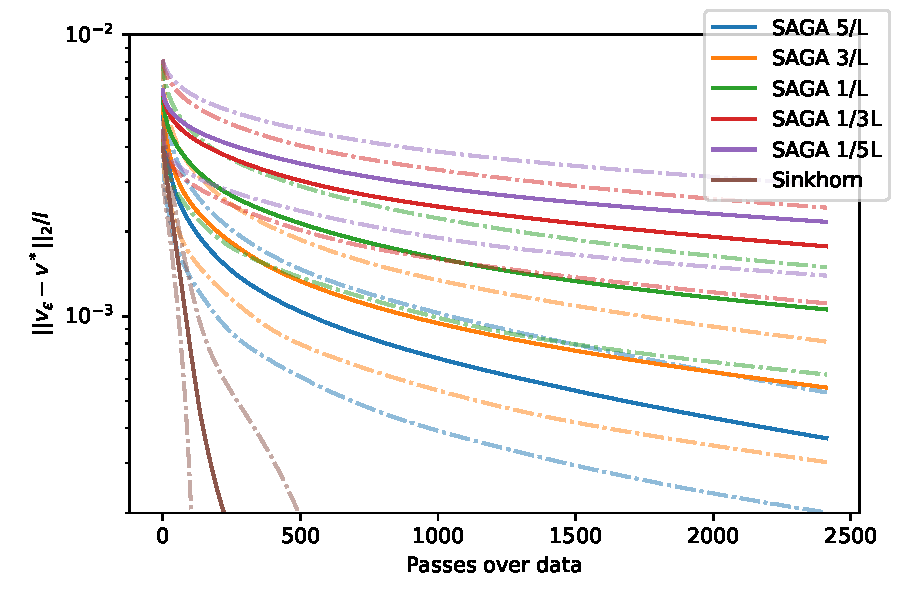
\includegraphics[width=\linewidth]{figures/saga_image_retreival_vs_avg.pdf}
        \end{figure}
    \end{minipage}
\end{frame}

\begin{frame}{Numerical findings - Semi-discrete OT}
    \begin{minipage}{.49\linewidth}
        \begin{figure}
            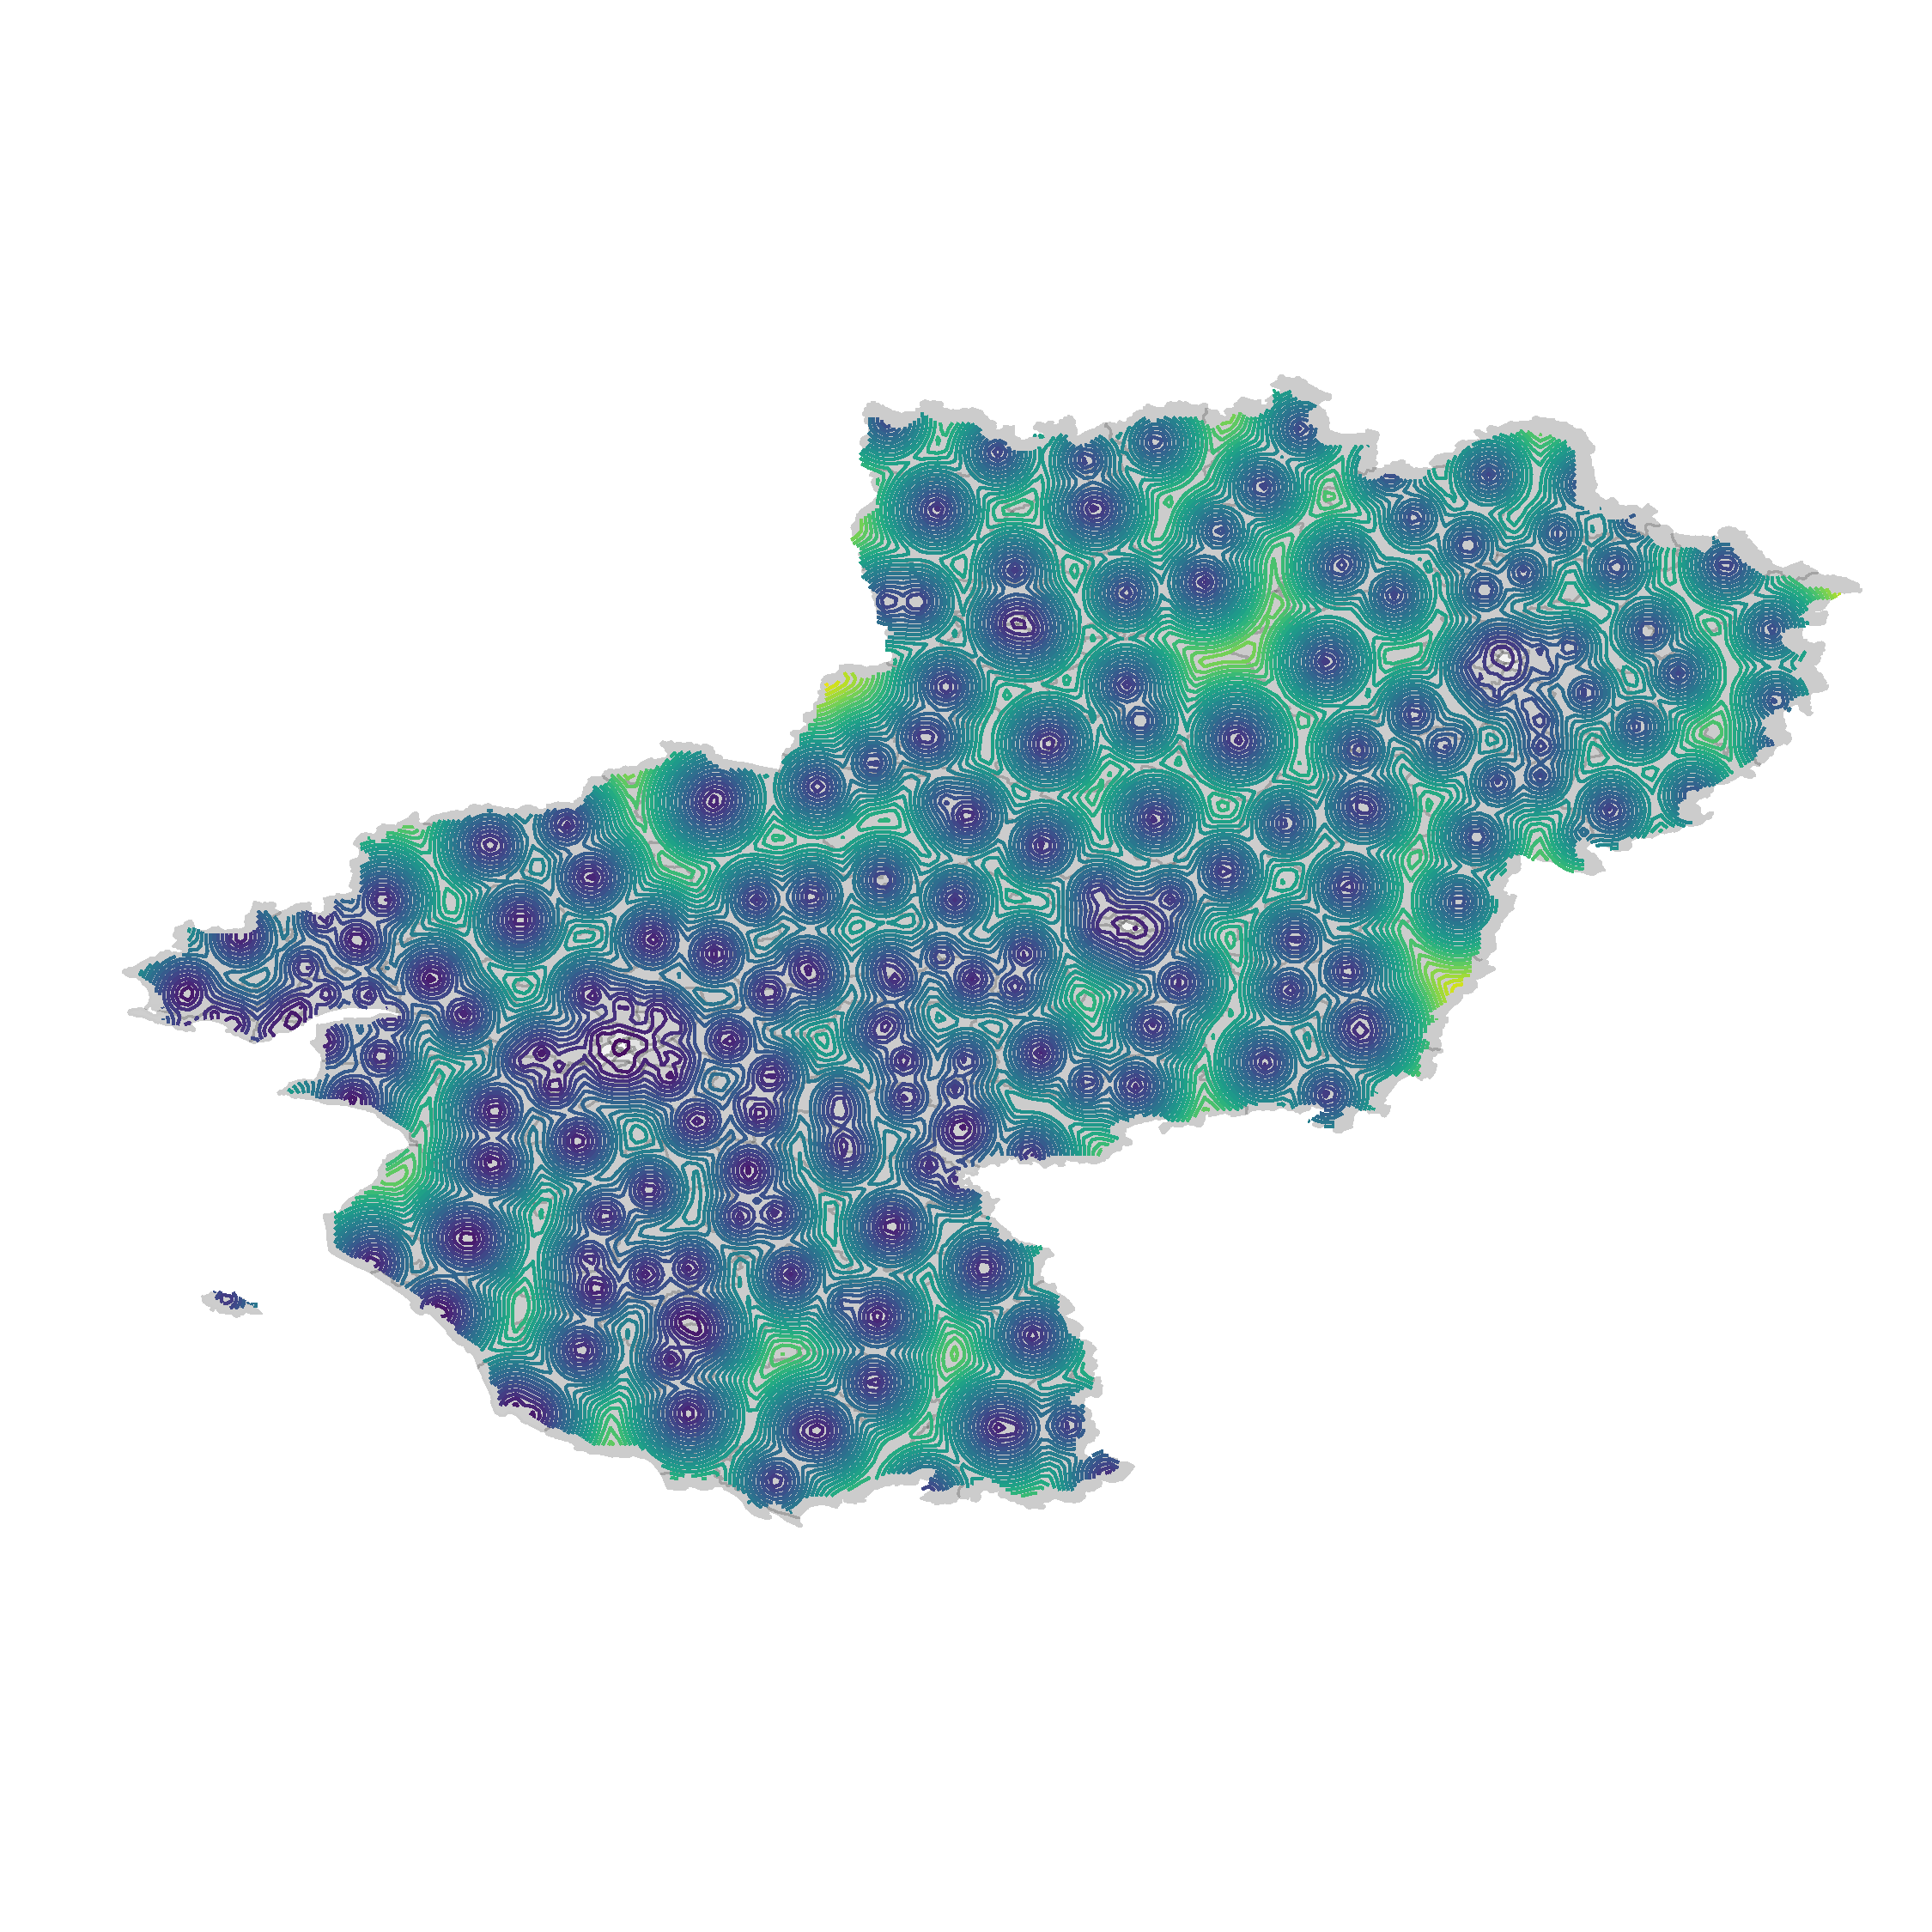
\includegraphics[width=.7\linewidth]{figures/opti_nantes.pdf}
        \end{figure}
        \begin{figure}
            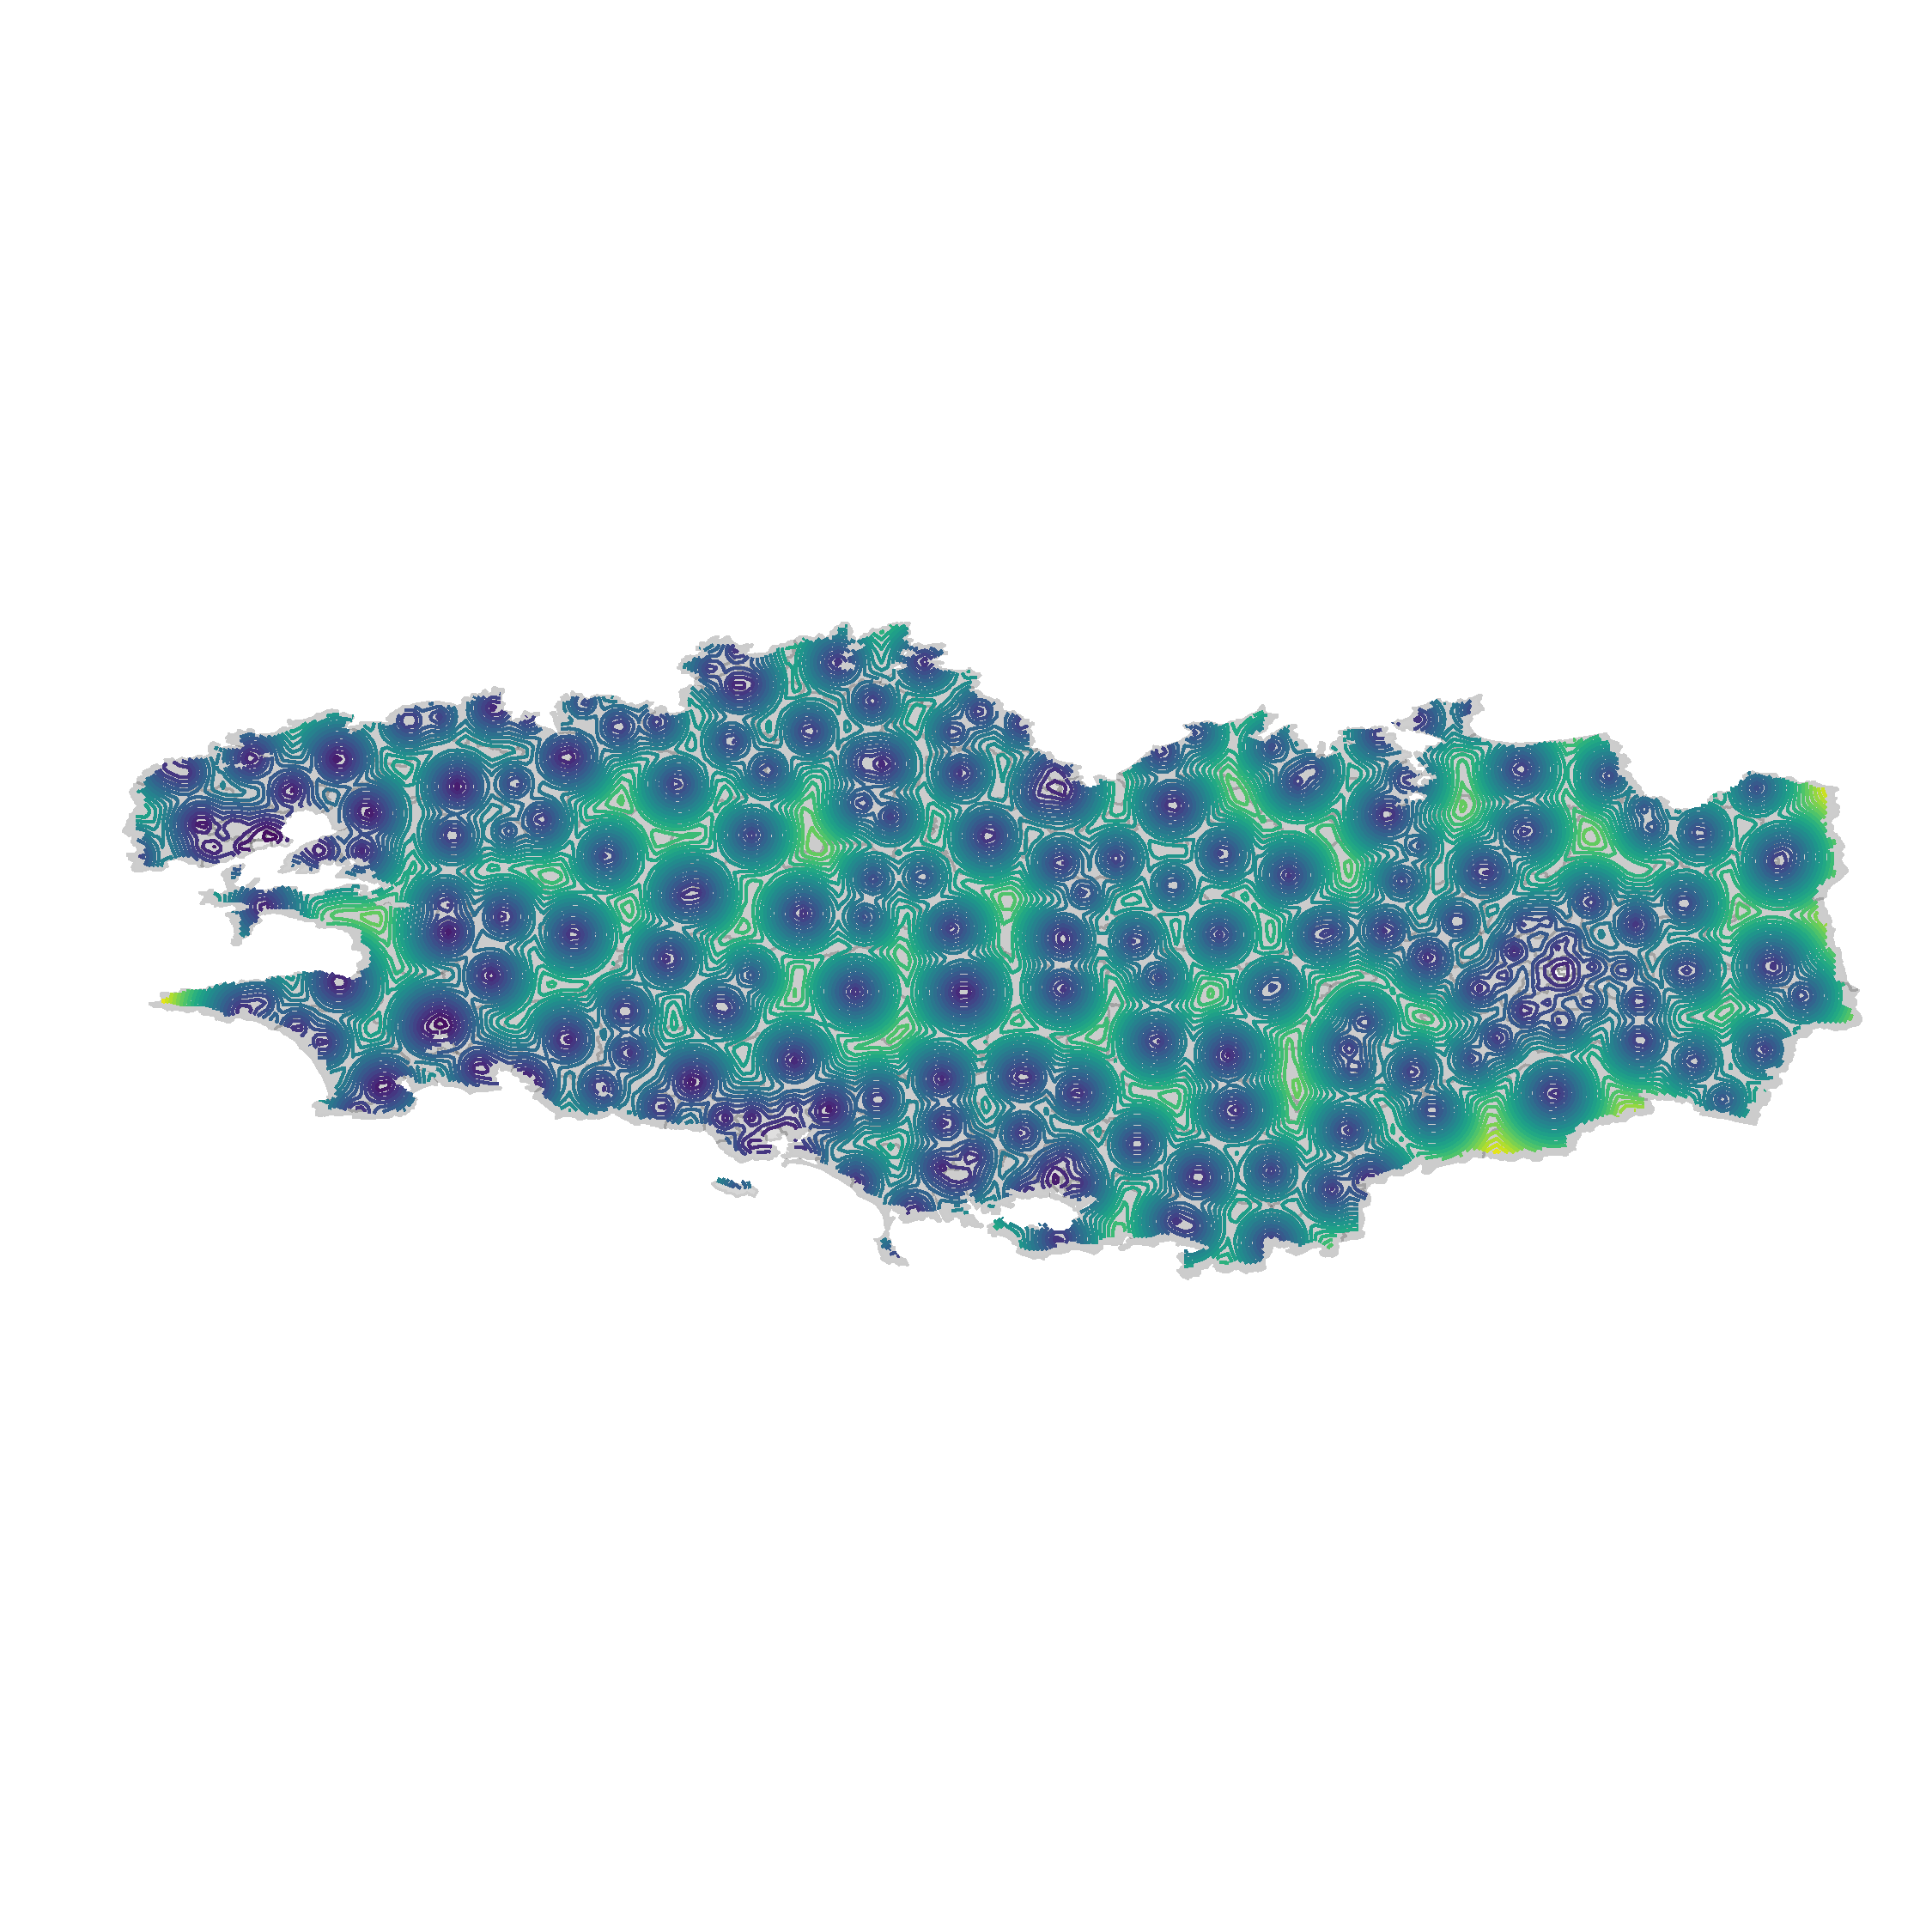
\includegraphics[width=.7\linewidth]{figures/opti_rennes.pdf}
        \end{figure}
    \end{minipage}
    \begin{minipage}{.49\linewidth}
        \begin{figure}
            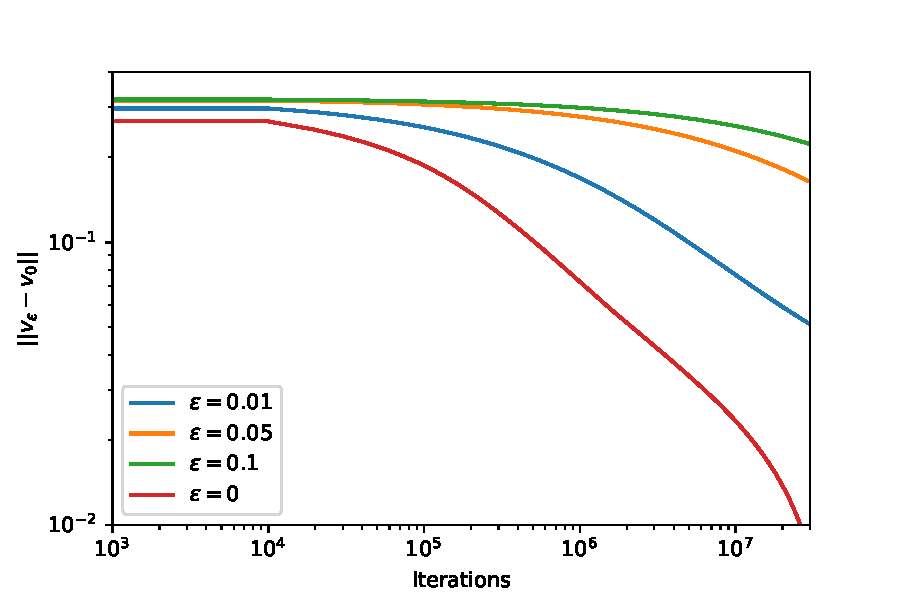
\includegraphics[width=.9\linewidth]{figures/semi_discrete_eps.pdf}
        \end{figure}
        \begin{figure}
            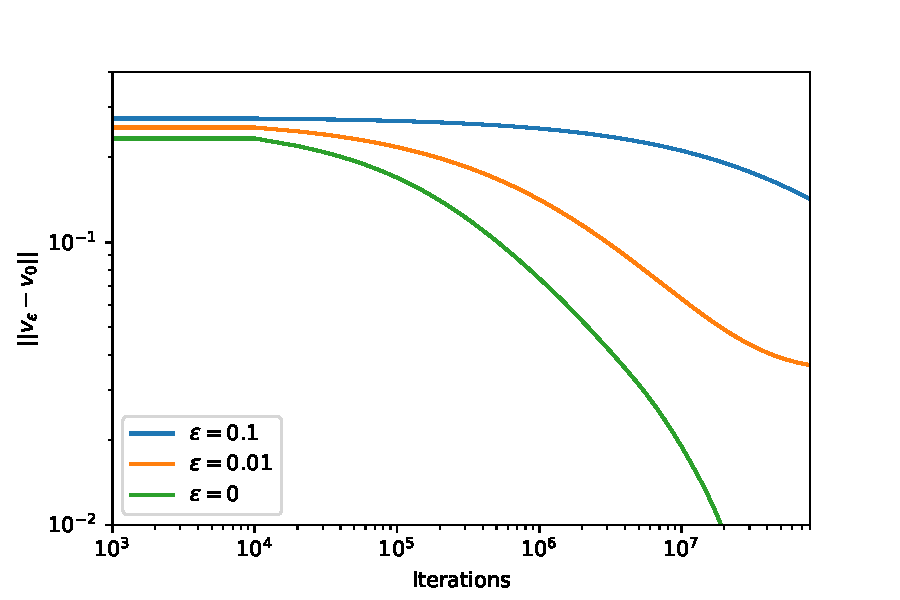
\includegraphics[width=.9\linewidth]{figures/semi_discrete_eps2.pdf}
        \end{figure}
    \end{minipage}
\end{frame}

\begin{frame}{Critics}
    \begin{itemize}
        \item These methods should be tested in a much larger scale setting to show their real benefit
        \item Benefits over Sinkhorn of SAG and SAGA wasn't consistently observed and seems to depend on the parameters and structure of the problem
    \end{itemize}
\end{frame}

\begin{frame}{Perspective}
    \begin{itemize}
        \item Applications of OT to problems with scales of the order of $10^6$ and above
        \item Applications of semi-discrete OT to high dimensional problems with ``exotic'' cost functions
    \end{itemize}
\end{frame}

\end{document}